\documentclass[11pt]{article}

\usepackage[T1]{fontenc}
\usepackage{lmodern}
\usepackage[margin=1in]{geometry}
\usepackage{amsmath,amssymb,amsthm}
\usepackage{mathtools}
\usepackage{enumitem}
\usepackage{booktabs}
\usepackage{xcolor}
\usepackage{tikz}
\usetikzlibrary{positioning,arrows.meta,fit}
\usepackage[colorlinks=true,linkcolor=blue,citecolor=blue,urlcolor=blue]{hyperref}

% ---------- palette (matches the project site and slides) ----------
\definecolor{ink}{RGB}{24,32,40}
\definecolor{trust}{RGB}{21,110,84}
\definecolor{agent}{RGB}{70,84,156}
\definecolor{flag}{RGB}{179,55,43}
\definecolor{muted}{RGB}{90,100,114}
\definecolor{paper}{RGB}{246,247,244}
\definecolor{trustwash}{RGB}{233,242,236}
\definecolor{agentwash}{RGB}{237,239,248}

\newcommand{\GF}{\mathbb{F}_2}
\newcommand{\HX}{H_X}
\newcommand{\HZ}{H_Z}
\newcommand{\rank}{\operatorname{rank}}
\newcommand{\wt}{\operatorname{wt}}
\newcommand{\supp}{\operatorname{supp}}
\newcommand{\diam}{\operatorname{diam}}
\newcommand{\eff}{kd^2/n}
\newcommand{\geff}{4kd^2/(n\rho^2 r^4)}

\title{\textbf{The QEC Challenge}\\[4pt]
	\large A public, automatically verified leaderboard for quantum
	low-density parity-check codes}
\author{Unitary Foundation \and
	\texttt{github.com/unitaryfoundation/qldpc-challenge}}
\date{\vspace{-2ex}\today}

\begin{document}
	\maketitle

	\begin{abstract}
		The QEC Challenge is a public leaderboard for quantum low-density
		parity-check codes. A participant submits a single JSON file describing
		one code --- a CSS code, or since schema 0.4 a general stabilizer code
		--- and continuous integration recomputes the code's properties,
		actively tries to refute its distance claim, and merges onto the board
		only a code that holds up. Three principles shape the design.
		(i) \emph{Everything cheap is trustless and mandatory}: the verifier
		recomputes $n$, $k$, commutation, connectivity, check weight, and the
		geometric locality class from scratch over $\GF$ --- a wrong claimed
		$k$ or a non-commuting ``stabilizer'' is rejected in milliseconds. (ii)
		\emph{Distance is layered by how much is proven}: a submitter attaches
		an explicit logical-operator \emph{witness} that proves
		$d\le\text{value}$ with no trust required; an adversarial
		\emph{refutation gate} then searches for a lighter logical, and
		separate certification tiers upgrade a claim to \emph{corroborated} or
		\emph{exact}. The same discipline extends to the circuit level: an
		entry may ship its syndrome-extraction circuits and claim a
		witnessed circuit-level distance and a measured logical error rate,
		both re-derived and re-measured by CI. (iii) \emph{A code is not a
		single number}: the primary tracks are a grid of \emph{computed} axes
		(locality class $\times$ check-weight class, with CSS and general
		stabilizer codes on separate boards), and within each cell the
		ranking is a Pareto frontier over $(n,k,d,w)$ rather than a scalar;
		two efficiency figures --- the \emph{operational} efficiency $\eff$
		and, for codes shipping a verified layout, the \emph{geometric}
		efficiency $g=\geff$, normalized so the planar surface code scores
		exactly $1$ --- are reported alongside the frontier, never in place
		of it. The whole pipeline --- validator, refutation gate, certifiers,
		circuit-tier verifier, scorer, static-site generator --- lives in the
		repository and runs in CI on every pull request, which also makes the
		board usable as the verification harness of automated (LLM- and
		agent-driven) code-discovery loops. As of 1 October 2026 the board
		holds 1791 verified codes, 625 of them certified exact.
	\end{abstract}

	\section{Overview}

	A submission is one JSON file placed under \texttt{codes/}, conforming to
	\texttt{schema/code.schema.json} (described in \texttt{schema/SCHEMA.md}). A
	contributor opens a pull request adding the file (one new code per PR,
	enforced by CI; an entry's circuit artifacts count as part of the same
	submission); GitHub Actions runs the verifier
	(\texttt{verify/qldpc\_verify.py}) and the distance refutation gate
	(\texttt{verify/gate\_changed.py}), and a green check means the code's
	cheap properties are confirmed \emph{and} an adversarial search failed to
	find a logical lighter than the claimed distance. After merge,
	\texttt{site/build.py} regenerates the static leaderboard into
	\texttt{docs/} automatically (an index with per-cell Pareto tables and
	plots, a separate board for general stabilizer codes, a logical-error-rate
	frontier, a page per code, a reference list, and status badges). The board
	is seeded with literature baselines --- the planar open-boundary codes of
	Liang, Eberhardt, and Chen~\cite{liang2025planar}, the bivariate-bicycle
	gross code~\cite{bravyi2024high}, generalized-bicycle
	codes~\cite{panteleev2021degenerate,wang2022distance}, coset
	codes~\cite{aydin2026breaking}, the non-abelian lifted-product mitten
	codes~\cite{bhardwaj2026mitten}, and the surface, toric, and Steane
	codes~\cite{kitaev2003fault,steane1996error} --- so a new entry is always
	measured against published codes rather than an empty board.

	Two things are deliberately \emph{not} asked of the submitter: a proof
	that their distance is exact (that is the server's job), and a single
	headline rank (the board is a Pareto frontier). Everything else --- the
	parity checks, the claimed $n,k,d$ with witnesses, an optional layout, an
	optional circuit tier, and provenance --- is supplied and then
	recomputed, witnessed, or attacked by the verifier.

	\begin{figure}[h]
	\centering
	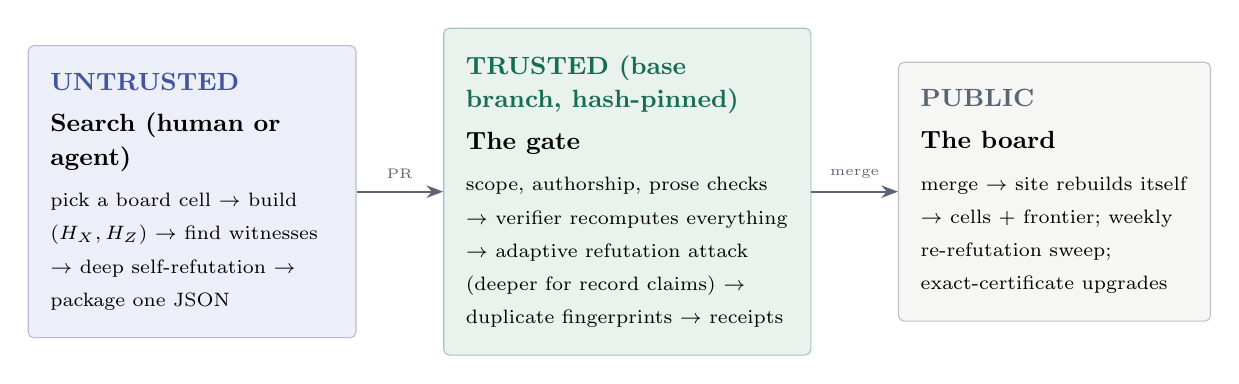
\begin{tikzpicture}[
		zone/.style={rounded corners=2pt, inner sep=8pt},
		arr/.style={-{Stealth[length=6pt]}, thick, muted}]
		\node[zone, fill=agentwash, draw=agent!40] (a) at (0,0)
			{\begin{minipage}{3.6cm}\raggedright\vspace{2pt}
			{\color{agent}\bfseries\small UNTRUSTED}\\[3pt]
			{\bfseries\small Search (human or agent)}\\[3pt]
			{\scriptsize pick a board cell $\to$ build $(\HX,\HZ)$ $\to$
			 find witnesses $\to$ deep self-refutation $\to$
			 package one JSON}\vspace{2pt}\end{minipage}};
		\node[zone, fill=trustwash, draw=trust!40, right=1.1cm of a] (b)
			{\begin{minipage}{4.1cm}\raggedright\vspace{2pt}
			{\color{trust}\bfseries\small TRUSTED (base branch, hash-pinned)}\\[3pt]
			{\bfseries\small The gate}\\[3pt]
			{\scriptsize scope, authorship, prose checks $\to$ verifier
			 recomputes everything $\to$ adaptive refutation attack (deeper
			 for record claims) $\to$ duplicate fingerprints $\to$
			 receipts}\vspace{2pt}\end{minipage}};
		\node[zone, fill=paper, draw=muted!40, right=1.1cm of b] (c)
			{\begin{minipage}{3.4cm}\raggedright\vspace{2pt}
			{\color{muted}\bfseries\small PUBLIC}\\[3pt]
			{\bfseries\small The board}\\[3pt]
			{\scriptsize merge $\to$ site rebuilds itself $\to$ cells +
			 frontier; weekly re-refutation sweep; exact-certificate
			 upgrades}\vspace{2pt}\end{minipage}};
		\draw[arr] (a) -- node[above=1pt, font=\tiny, muted] {PR} (b);
		\draw[arr] (b) -- node[above=1pt, font=\tiny, muted] {merge} (c);
	\end{tikzpicture}
	\caption{Three zones, one direction of trust. A submission originates in
	an untrusted search (increasingly, an automated one), is judged entirely
	by pinned code running from the base branch, and only then becomes part of
	the public record --- which keeps being re-attacked after merge.}
	\label{fig:zones}
	\end{figure}

	\section{Why a leaderboard of cells, not one number}

	A quantum code trades several quantities against one another --- physical
	qubits $n$, logical qubits $k$, distance $d$, maximum check weight $w$, and
	geometric locality --- and separately has a decoding performance.
	Collapsing all of that into one scalar would reward gaming one axis at the
	expense of the rest. So the board is stratified in three layers
	(\texttt{TRACKS.md}).

	\paragraph{Layer 1: primary tracks, computed, never self-declared.} The
	primary tracks are a grid of two nested axes whose membership is
	\emph{derived by the verifier} from the parity checks and the layout, so a
	track cannot be claimed by relabeling:
	\begin{itemize}[nosep]
		\item a \textbf{locality class}: \texttt{local-2d-single} (one layer,
		interaction radius $\le 4$) $\subset$ \texttt{local-2d-bilayer} (up to
		two layers --- the flip-chip regime --- radius $\le 7$) $\subset$
		\texttt{unrestricted} (everything else, including any code without a
		layout and any three-dimensional layout);
		\item a \textbf{check-weight class}: \texttt{weight-4} $\subset$
		\texttt{weight-6} $\subset$ \texttt{weight-8} $\subset$ any weight,
		from the maximum row weight of $\HX,\HZ$ (for a general stabilizer
		code, the number of qubits a generator acts on, a $Y$ counting once).
	\end{itemize}
	The classes nest: a single-layer weight-4 code also competes on every
	looser board. Each (locality, weight) cell is a board of its own
	(Figure~\ref{fig:grid}). The code type is a third cell dimension: CSS
	codes and general stabilizer codes are ranked on separate leaderboards
	with the same grid, because $\eff$ does not mean the same thing for
	both --- the two families decode differently, and how the figure tracks
	a logical error rate is less settled for non-CSS codes. A stabilizer
	code never dominates or is dominated by a CSS entry.

	\begin{figure}[h]
	\centering
	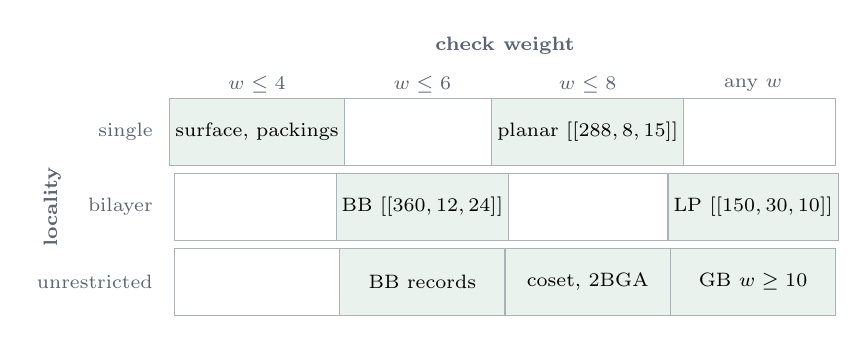
\begin{tikzpicture}[
		cell/.style={draw=muted!50, minimum width=2.1cm, minimum height=0.85cm,
		             font=\scriptsize, inner sep=2pt}]
		\node[font=\scriptsize\bfseries, muted] at (3.15, 3.0) {check weight};
		\foreach \j/\wl in {0/{$w\le4$}, 1/{$w\le6$}, 2/{$w\le8$}, 3/{any $w$}}
			\node[font=\scriptsize, muted] at (2.1*\j, 2.5) {\wl};
		\node[font=\scriptsize\bfseries, muted, rotate=90] at (-2.6, 0.95) {locality};
		\foreach \i/\ll in {0/{single}, 1/{bilayer}, 2/{unrestricted}}
			\node[font=\scriptsize, muted, anchor=east] at (-1.2, 1.9-0.95*\i) {\ll};
		\foreach \j in {0,...,3} \foreach \i in {0,...,2}
			\node[cell] at (2.1*\j, 1.9-0.95*\i) {};
		\node[cell, fill=trustwash] at (0, 1.9) {surface, packings};
		\node[cell, fill=trustwash] at (4.2, 1.9) {planar $[[288,8,15]]$};
		\node[cell, fill=trustwash] at (2.1, 0.95) {BB $[[360,12,24]]$};
		\node[cell, fill=trustwash] at (6.3, 0.95) {LP $[[150,30,10]]$};
		\node[cell, fill=trustwash] at (2.1, 0.0) {BB records};
		\node[cell, fill=trustwash] at (4.2, 0.0) {coset, 2BGA};
		\node[cell, fill=trustwash] at (6.3, 0.0) {GB $w\ge 10$};
	\end{tikzpicture}
	\caption{The primary-track grid: locality class $\times$ check-weight
	class, both computed from the submission (example occupants of the CSS
	board shown). Within each cell the ranking is the Pareto frontier over
	$(n,k,d,w)$; a code in a tight cell also competes in every looser cell
	it nests into. The general-stabilizer board has the same grid.}
	\label{fig:grid}
	\end{figure}

	\paragraph{Layer 2: family tags, filterable, never ranked.} The
	construction family (bivariate bicycle, generalized bicycle --- including
	non-abelian two-block group-algebra
	constructions~\cite{lin2024quantum} --- coset, lifted product, tile,
	topological, \dots) cannot be recovered from the matrices, so it is a
	self-reported, filterable tag that confers no ranking advantage.

	\paragraph{Layer 3: verified flags.} Only properties a verifier or a
	certificate can prove: CSS commutation (or, for a general stabilizer
	code, that its generators commute), the locality class (which doubles
	as Layer-1 membership), \texttt{modular} (the layout assigns every qubit
	to a hardware module), and the distance-confidence tier of
	Section~\ref{sec:distance}.

	\paragraph{Diagnostics, displayed but never ranked.} The verifier also
	reports properties that no track reads: the girth of each side's Tanner
	graph, the row and column weight profiles, a census of small trapping
	sets, the Euclidean support diameter of each stored distance witness for
	a laid-out code, and a heuristic routing cost (nearest-neighbour SWAPs
	per syndrome-extraction round to connect every check's support on the
	shipped layout --- a minimum-spanning-tree lower bound, not a schedule).
	They appear on code pages and as sortable columns; they enter neither
	the frontier nor any score.

	\paragraph{Pareto frontier, not a single winner.} Within a cell, a code is
	a record if no other code in the cell dominates it --- no other has
	$n'\le n$, $k'\ge k$, $d'\ge d$, $w'\le w$ with at least one strict
	inequality. There can be many co-leaders. A record whose \emph{only}
	strict axis is $d$ is a different kind of claim: both numbers are
	witness-backed upper bounds, so the comparison says which search ran
	deeper as much as which code is better, and this is where the board has
	historically been wrong ($[[882,18,30]]\to 29$, $[[684,12,81]]\to 66$).
	The gate reports that pattern explicitly, naming the entry that was
	beaten, so that it can be re-measured at matched depth.

	\paragraph{Efficiency as sortable columns, not the rank.} Two efficiency
	figures are reported per cell and sortable, but neither collapses the
	frontier into one number: the \emph{operational} efficiency $\eff$ used
	by the 2D-locality literature, and the \emph{geometric} efficiency $g$
	of Section~\ref{sec:geff}, which additionally prices the layout a code
	ships with. Both are monotone in $d$, so a code whose distance is only
	an upper bound carries the one $d\le$ marker in the distance column
	that governs both.

	\section{Background: two efficiency metrics and the BPT bound}

	For an $[[n,k,d]]$ stabilizer code, the Bravyi--Poulin--Terhal (BPT) bound~\cite{bravyi2010tradeoffs}
	states that any geometrically 2D-local code obeys
	\begin{equation}
		\frac{kd^2}{n} \;\le\; c(r,w,q),
		\label{eq:bpt}
	\end{equation}
	where the constant $c$ depends only on the interaction range $r$, the
	maximum stabilizer weight $w$, and the on-site dimension $q$ --- not on
	$n$. The optimal constant is open, which makes ``within a fixed locality
	model, maximize $\eff$'' a well-posed target for the 2D-local cells. For
	asymptotically good codes~\cite{panteleev2022asymptotically,tillich2014quantum}, where $k$ and $d$ both grow linearly with $n$,
	$\eff$ grows like $n^2$ without bound --- which is exactly why the board
	buckets and compares like with like rather than ranking a
	$[[120,\dots]]$ entry against a $[[10^4,\dots]]$ one. Reference points
	from the literature, spanning the efficiency range (all $q=2$; $w$ = max
	check weight):
	\begin{center}
		\begin{tabular}{lcccc}
			\toprule
			Code & $[[n,k,d]]$ & topology & $w$ & $\eff$\\
			\midrule
			Rotated planar surface~\cite{kitaev2003fault} & $[[d^2,1,d]]$ & planar & 4  & $1$\\
			Gross code (IBM)~\cite{bravyi2024high} & $[[144,12,12]]$ & periodic & 6  & $12$\\
			Tile code~\cite{steffan2025tile} & $[[512,18,19]]$ & planar & 8  & $12.7$\\
			Generalized bicycle~\cite{panteleev2021degenerate} & $[[126,28,8]]$ & periodic & 10 & $14.2$\\
			Coset two-block~\cite{aydin2026breaking} & $[[168,20,14]]$ & unrestricted & 8  & $23.3$\\
			Mitten (lifted product)~\cite{bhardwaj2026mitten} & $[[540,108,18]]$ & unrestricted & 9 & $64.8$\\
			\bottomrule
		\end{tabular}
	\end{center}
	The planar rows are the open-boundary program of Liang, Eberhardt, and
	Chen~\cite{liang2025planar} and the tile codes~\cite{steffan2025tile};
	the coset row is the two-block generalization of Aydin, Tamo, and
	Barg~\cite{aydin2026breaking}; the mitten and ZSZ-LP
	families~\cite{bhardwaj2026mitten,hong2026zszlp} reach rate $1/5$ at
	weight 9 by two different non-abelian routes. Whether planar codes can
	close the gap to the periodic and unrestricted records is the kind of
	question a live leaderboard can resolve.

	\subsection{Geometric efficiency: pricing the layout}
	\label{sec:geff}

	Operational efficiency deliberately ignores \emph{how} a code is laid
	out: a periodic code and a planar code with the same $[[n,k,d]]$ score
	the same $\eff$, although one assumes long-range couplers the other does
	not need. The board therefore also reports, for every code whose layout
	the verifier has accepted, a \emph{geometric} efficiency that prices the
	layout itself:
	\begin{equation}
		g \;=\; \frac{4\,kd^2}{n\,\rho^2\,r^4},
		\label{eq:geff}
	\end{equation}
	where $r$ is the \emph{measured} interaction radius of the shipped
	layout (the maximum Euclidean check diameter, in units of the unit qubit
	spacing) and $\rho$ its layer count. This is the BPT
	ratio~\eqref{eq:bpt} charged for its geometric resources: the $r^4$
	factor is the range dependence of the BPT constant in 2D, and $\rho^2$
	is the unique exponent that makes re-packaging a layout into layers
	score-neutral, so $g$ cannot be inflated by stacking. The constant
	$4=(\sqrt2)^4$ normalizes the rotated planar surface code ($r=\sqrt2$,
	$\rho=1$) to exactly $g=1$, which gives the figure an absolute meaning:
	a code family that sustains $g>1$ at growing distance packs more
	protected logical content per qubit under the \emph{same} hardware
	locality budget as the surface code. A layout may also carry
	three-dimensional coordinates; the BPT bound in $D$ dimensions is
	$kd^{2/(D-1)}=O(n)$, and the same coarse-graining gives
	$g=2\sqrt2\,kd/(n\rho r^3)$ for $D=3$, normalized so a code saturating
	$kd=n$ at the nearest-neighbour cubic radius $r=\sqrt2$ scores $1$. A 3D
	layout earns no 2D-local class and $g$ is compared within a dimension,
	never across.

	Three design details keep $g$ honest. It is computed only from a
	verifier-accepted layout (Section~\ref{sec:checks}, V9) --- $r$ and
	$\rho$ are recomputed from the shipped coordinates, never taken from the
	submission --- and a code without a layout simply has no $g$, which is a
	certification status rather than a judgment. Constant-distance tilings
	exceed $g=1$ trivially (a $[[4,2,2]]$ block on one plaquette scores
	$g=2$), so the board's headline figure requires $d\ge 3$. And $g$
	inherits the distance tier: computed from an upper-bound $d$ it is an
	upper bound.

	When the first version of this document was written, the rotated surface
	codes held the ceiling at $g=1$ and the best contributed layout reached
	$g\approx0.38$. That is no longer the state of the board. Multi-band
	dense packings of surface-code patches on a shared plane, generalizing
	the code-deformation procedures of Fujiu, Nagayama, Nishio, Kawaguchi,
	and Satoh (\texttt{arXiv:2511.06758}), keep the surface code's own
	weight-4 checks and $r=\sqrt2$ radius while sharing boundary ancillas
	between patches, and they now exceed $g=1$ at every distance the board
	has them at: $g=1.68$ at $d=3$ ($[[925,173,3]]$), $1.35$ at $d=5$
	($[[998,54,5]]$), $1.31$ at $d=7$, $1.29$ at $d=9$ (the $[[691,11,9]]$
	member is certified exact), and $1.27$ at $d=13$ ($[[931,7,13]]$). The
	sequence decreases slowly with $d$, which turns the open question of
	Section~\ref{sec:open} from ``can any layout beat $1$'' into ``where does
	this family's $g$ converge, and does the advantage survive at the
	circuit level, where the shared ancillas also share hook errors''.

	\section{Submission format}

	A submission is one JSON object (\texttt{schema\_version} \texttt{"0.1"}
	through \texttt{"0.4"}; \texttt{code\_type} \texttt{"CSS"} or
	\texttt{"stabilizer"}) with:
	\begin{itemize}[nosep]
		\item \texttt{n} --- physical qubit count; must match the indices used
		in \texttt{checks}. Admissible blocklengths are $n\le 700$, or
		$n\le 1000$ when the maximum check weight is $\le 8$ and the claimed
		$d\le 40$ --- a verification-budget rule, since the refutation gate
		must be able to search meaningfully behind every claim in CI.
		\item \texttt{k} --- \emph{claimed} logical qubit count; the verifier
		recomputes it and requires an exact match.
		\item \texttt{checks.X}, \texttt{checks.Z} --- the parity checks as
		sparse supports: each is a list of checks, each check a sorted list of
		distinct $0$-based qubit indices. A general stabilizer code instead
		ships \texttt{checks.S}, a list of generators each given as an $X$
		support and a $Z$ support (a qubit in both carries $Y$); this is the
		binary symplectic matrix $S=(A\,|\,B)$.
		\item \texttt{distance.d} --- claimed distance $=\min(d_X,d_Z)$, and
		per side \texttt{distance.X}/\texttt{distance.Z}, each a
		$\{\texttt{value},\texttt{confidence},\texttt{witness}\}$ triple,
		where \texttt{confidence} is \texttt{"upper\_bound"} or
		\texttt{"exact"} and \texttt{witness} is the support of a logical
		operator of that Pauli type and weight \texttt{value}. A stabilizer
		code has no sides: it carries a single \texttt{distance.P} whose
		witness is one Pauli operator and whose \texttt{value} is its Pauli
		weight.
		\item \texttt{locality} (optional) --- \texttt{coordinates} (one
		$[x,y]$ or $[x,y,z]$ per qubit), \texttt{layers} (required with a
		layout), and optionally \texttt{modules} (one hardware-module id per
		qubit); the verifier recomputes the interaction radius and derives
		the locality class from it. A missing layout is not an error --- the
		code simply competes as \texttt{unrestricted} --- but a dishonest one
		(crammed sites, or sites closer than the unit spacing) fails
		verification, and an honest layout above every class cap is demoted
		to \texttt{unrestricted} through a named check rather than silently.
		\item \texttt{circuit} (optional; RFC 0001) --- the circuit tier. The
		entry additionally ships memory experiments under
		\texttt{circuits/<slug>/} (\texttt{memory\_x.stim},
		\texttt{memory\_z.stim}, and their derived detector error models
		\texttt{.dem}) and claims a per-basis circuit-level distance
		\texttt{d\_circ} with a witness, a round count $\ge d$, and the pinned
		\texttt{stim} version. It may also carry \texttt{gates}, claimed
		transversal Clifford gates, and \texttt{ler}, a measured logical error
		rate (Section~\ref{sec:circuit}).
		\item \texttt{provenance} --- \texttt{authors} (the humans, by GitHub
		handle; the PR author must be listed), \texttt{construction} (a
		reproducible recipe), optional \texttt{references}, \texttt{date},
		\texttt{notes}, an optional literature-\texttt{novelty} status (a
		submitter claim), an optional \texttt{search\_budget} (what the
		search cost), and an optional \texttt{model} field naming the AI
		system that produced the code, to a specific version ---
		machine-discovered entries are attributed as such.
		\item \texttt{witness\_provenance} (optional, schema 0.2) --- who found
		the stored witnesses and how, including a \emph{survival stamp}: the
		number of independent refutation samples the claim has survived.
		Refutation credit lives on the witness, not on the code's author list,
		so a tightening correction by a third party never rewrites authorship.
	\end{itemize}
	(A legacy self-declared \texttt{tracks} field is deprecated and ignored
	for ranking; track membership is computed.) Verify locally before opening
	the PR (the project uses \texttt{uv}):
	\begin{center}
		\texttt{uv run python verify/qldpc\_verify.py codes/your-code.json}
	\end{center}
	The verifier prints a JSON report --- per-check pass/fail, the computed
	$n$, $k$, ranks, weight class, locality class, diagnostics --- and an
	\texttt{earned\_distance} block giving the tier each side actually
	earned, and exits $0$ iff every required check passes. The \texttt{cli/}
	launcher automates the whole path: \texttt{./qldpc submit} turns
	parity-check or symplectic matrices (however constructed --- e.g.\ with
	the \texttt{qLDPC} library~\cite{perlin2023qldpc}) into a verified,
	PR-ready file, generating and verifying the circuit tier by default;
	\texttt{./qldpc targets} lists which track cells are open and what a
	code of a given size needs to enter them; \texttt{./qldpc recent}
	summarizes what landed lately; and \texttt{./qldpc reproduce} replays an
	entry from its reproduction manifest.

	\section{What the verifier checks}
	\label{sec:checks}

	A submission is rejected unless all of the following hold. Checks
	(V1)--(V10) are polynomial-time and run in CI on every PR; the refutation
	gate and the certification tiers (Section~\ref{sec:distance}) are layered
	on top.
	\begin{enumerate}[label=(V\arabic*),leftmargin=*,nosep]
		\item \textbf{Schema and indices.} The document conforms to
		\texttt{code.schema.json}, every qubit index in \texttt{checks} is in
		$[0,n)$, the blocklength is admissible, and the file is within size
		limits.
		\item \textbf{No collapsed checks.} No qubit index is repeated within
		a single check (a repeat would XOR away and silently change the code).
		\item \textbf{Commutation.} $\HX\HZ^{\!\top}=0$ over $\GF$ for a CSS
		code; isotropy $AB^{\top}+BA^{\top}=0$ for a general stabilizer code.
		A submission typed \texttt{stabilizer} whose every generator is pure
		$X$ or pure $Z$ is a CSS code and is rejected until typed as one.
		\item \textbf{Connectivity.} The Tanner graph is connected, and ---
		because a redundant row spanning two blocks can join the graph without
		changing the code --- so is the Tanner graph of the reduced row
		echelon form of the checks: the stabilizer group must not be a direct
		sum over disjoint qubit sets. A direct sum of two board codes is not a
		new code; the echelon-form check closed the redundant-row evasion
		that was tried against the first version of the test.
		\item \textbf{Logical dimension.} The verifier recomputes
		$k = n-\rank_{\GF}(\HX)-\rank_{\GF}(\HZ)$ (or $k=n-\rank S$),
		requires it to equal the claimed $k$, and requires $k\ge 1$.
		\item \textbf{LDPC weight cap and vocabulary.} The maximum check
		weight is bounded (the board is for LDPC codes), the family tag is
		from the controlled vocabulary, and a \texttt{model} field names a
		specific version.
		\item \textbf{Distance witnesses.} For each provided side, the witness
		$v$ must (a) have weight equal to the claimed \texttt{value}, (b) lie
		in the kernel of the opposite checks (an $X$-witness commutes with
		$\HZ$; a Pauli witness commutes with every generator), and (c) be
		nontrivial, i.e.\ not in the rowspace of its own checks (not a
		stabilizer product). This certifies
		$d_{\text{side}}\le\texttt{value}$ as an \emph{upper bound} with no
		trust required.
		\item \textbf{Distance consistency.} The claimed $d$ equals the
		minimum over the witnessed sides.
		\item \textbf{Layout honesty and locality class (if a layout is
		present).} \texttt{coordinates} must cover all $n$ qubits; at most
		\texttt{layers} qubits may share a site and distinct sites must be
		$\ge 1$ apart (no cramming --- a small radius cannot be faked by
		collapsing qubits onto a point), and either violation fails the
		submission; the recomputed maximum check diameter then decides the
		class. The class is \emph{earned} from the layout, never declared.
		\item \textbf{Quick refutation.} A short random-information-set
		search must fail to find a logical lighter than the claim (the full
		gate of Section~\ref{sec:distance} runs far deeper).
	\end{enumerate}
	Every \texttt{exact} confidence claim is \emph{downgraded to
	upper\_bound here} and flagged for server certification --- the cheap PR
	check never upgrades a distance to exact. The verifier also files, with
	every CSS code, the fingerprints of its images under local Hadamards, so
	that a Hadamard-relabelled copy collides with it whichever code type it
	is submitted under.

	\section{Distance: three tiers and an adversarial gate}
	\label{sec:distance}

	The distance is the minimum weight over nontrivial logicals; for a CSS
	code $d=\min(d_X,d_Z)$, for a general stabilizer code the minimum Pauli
	weight. The problem is NP-hard~\cite{kapshikar2023hardness}, and the
	hardness is asymmetric: exhibiting a low-weight logical gives only an
	\emph{upper} bound, while certifying $d\ge D$ is the hard direction ---
	and a submitter has every incentive to overclaim. Heuristic distance
	estimates routinely deflate under deeper search, so the challenge layers
	three confidence tiers (Figure~\ref{fig:tiers}) behind an active gate.

	\begin{figure}[h]
	\centering
	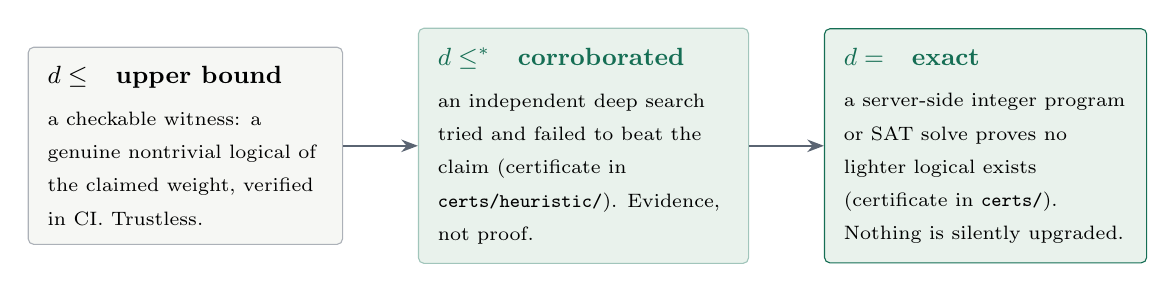
\begin{tikzpicture}[
		tier/.style={rounded corners=2pt, inner sep=7pt},
		arr/.style={-{Stealth[length=6pt]}, thick, muted}]
		\node[tier, fill=paper, draw=muted!50] (ub) at (0,0)
			{\begin{minipage}{3.5cm}\raggedright
			{\bfseries\small $d\le$ \; upper bound}\\[3pt]
			{\scriptsize a checkable witness: a genuine nontrivial logical of
			 the claimed weight, verified in CI. Trustless.}\end{minipage}};
		\node[tier, fill=trustwash, draw=trust!40, right=0.95cm of ub] (corr)
			{\begin{minipage}{3.7cm}\raggedright
			{\color{trust}\bfseries\small $d\le^{*}$ \; corroborated}\\[3pt]
			{\scriptsize an independent deep search tried and failed to beat
			 the claim (certificate in \texttt{certs/heuristic/}). Evidence,
			 not proof.}\end{minipage}};
		\node[tier, fill=trustwash, draw=trust, right=0.95cm of corr] (ex)
			{\begin{minipage}{3.6cm}\raggedright
			{\color{trust}\bfseries\small $d=$ \; exact}\\[3pt]
			{\scriptsize a server-side integer program or SAT solve proves no
			 lighter logical exists (certificate in \texttt{certs/}). Nothing
			 is silently upgraded.}\end{minipage}};
		\draw[arr] (ub) -- (corr);
		\draw[arr] (corr) -- (ex);
	\end{tikzpicture}
	\caption{The distance-confidence ladder. Every tier is backed by an
	artifact in the repository: a witness inside the submission, a heuristic
	certificate, or an exact certificate.}
	\label{fig:tiers}
	\end{figure}

	\paragraph{Upper-bound tier (trustless, in CI).} The submitter's witness
	is checked exactly as in (V7). A valid witness proves
	$d_{\text{side}}\le\texttt{value}$; the board labels such a code $d\le$
	and lets anyone climb instantly, since the arithmetic is checked rather
	than trusted.

	\paragraph{The refutation gate (adversarial, in CI).} Every changed code
	faces bounded searches for a logical \emph{lighter} than the claim. The
	gate is staged. A cheap \emph{structural} pass runs first: a circulant
	generalized-bicycle code, detected from its matrices rather than from
	its family tag, is attacked through its own block structure, which finds
	the low-weight logicals brute force misses. Then a random-information-set
	(RIS) search (randomized distance estimation in the spirit of
	\texttt{QDistRnd}~\cite{pryadko2023qdistrnd}) runs with an adaptive
	budget: trials scale with $n$, and a code that would enter a cell's
	Pareto frontier faces a much deeper battery than a dominated one, so
	over-claims pay extra scrutiny exactly where gaming would matter.
	Frontier claims additionally face an accelerated RIS pass (a bit-packed
	$\GF$ engine at roughly $150\times$ the baseline trial budget, capped at
	90 minutes of wall-clock) that only \emph{proposes} candidates: a find
	counts as a refutation solely after the pinned Python verifier validates
	the witness, so the extra depth adds no trust surface, and a missing or
	broken accelerator falls back to the full multi-seed Python battery
	rather than a shallower gate. A syndrome-decoder (BP+OSD) search ran
	alongside RIS for the board's first year and was retired in September
	2026 after a measured comparison showed it never found a logical the RIS
	search had not, at a small fraction of the trial rate. Any hit is a sound
	refutation --- it exhibits a checkable counterexample --- and fails the
	PR. The per-run seed is random by design, so an over-claim cannot be
	tuned to evade one fixed search; a weekly whole-board sweep re-runs the
	refutation with fresh seeds to accumulate coverage over time.

	The gate prices the \emph{diff}, not just the code. A layout-only change
	(checks and distance byte-identical to the base) skips refutation, since
	the claim already survived when it merged; a tightening correction
	(values strictly down, new witnesses of exactly the new weights) gets
	the standard shallow pass; a diff that adds or raises a survival stamp
	gets the deep battery regardless of record status, because a stamp is
	itself a claim that deters future refuters; anything else fails closed to
	the full search. The classification is recomputed from the git diff,
	never taken from the PR's framing, and every run leaves a verification
	receipt as a CI artifact.

	\paragraph{Corroborated tier.} A maintainer-run deep search
	(\texttt{verify/heuristic\_certify.py}) that tries and fails to beat a
	claim writes a heuristic certificate; the board then shows $d\le^{*}$.
	This is evidence, not proof --- the label records exactly how hard the
	claim has been attacked.

	\paragraph{Exact tier (server-certified).} To upgrade a side to $d=$, a
	maintainer proves no lighter nontrivial logical exists. Two certifiers
	ask the same question. \texttt{verify/certify.py} solves one bounded
	integer program per logical generator $t_L$ of the relevant type
	(scipy/HiGHS, no commercial solver): does a $v$ exist with
	\begin{equation}
		H v \equiv 0,\qquad \langle v,t_L\rangle\equiv 1 \pmod 2,\qquad
		\wt(v)\le \texttt{value}-1,
		\label{eq:milp}
	\end{equation}
	the mod-2 constraints linearized by integer slacks. Its cost is $k$
	solves per side, which is why it stalls on high-rate codes.
	\texttt{verify/sat\_certify.py} encodes the same question for a SAT
	solver with one selector variable per generator and a single clause
	requiring at least one anticommutation, so the whole side is one
	UNSAT proof instead of $k$; because that constraint set is invariant
	under the block rotations of two-block circulant codes, lex-leader
	symmetry breaking becomes legal and pays for itself at large $k$ (the
	$[[126,28,8]]$ generalized-bicycle code certifies in minutes where the
	per-generator form needed hours). If every
	generator on both sides is proven \emph{infeasible}, $d$ is exact; if a
	lighter logical is found, the claim is \emph{refuted}; if the solver
	hits its time limit, the side honestly remains an upper bound. A
	successful run writes a certificate to \texttt{certs/<slug>.json}, which
	is what upgrades a code's board label to $d=$. Exact records outrank
	equal upper-bound ones; nothing is ever silently upgraded. General
	stabilizer codes are not yet certified --- both certifiers minimize
	Hamming weight per side, not Pauli weight --- so every entry on that
	board is $d\le$.

	\section{The circuit tier: distance and error rate under a noise model}
	\label{sec:circuit}

	A code's distance is a property of its stabilizer group; what a device
	experiences is the distance of a particular syndrome-extraction
	\emph{circuit}, which hook errors and idle noise can lower well below
	$d$. The circuit tier (RFC 0001) transplants the code-tier discipline to
	that question. An entry ships memory experiments in \texttt{stim}'s
	circuit format for both bases, written in a canonical noise recipe at
	the reference rate $p=10^{-3}$ --- two-qubit depolarizing noise after
	every two-qubit gate, reset and measurement flips, and single-qubit
	depolarizing noise on every idle data qubit in every layer --- in which
	noise placement is not a submitter degree of freedom but the schedule
	is. Every \texttt{TICK} layer must be genuinely parallel (no qubit
	operated on twice), since the layer count sets the idle noise and
	deleting annotations would otherwise shed fault mechanisms. The
	verifier (\texttt{verify/circuit\_verify.py}) checks that the noiseless
	skeleton is deterministic, that the circuit equals its own re-noised
	skeleton, that the observables are the code's declared logicals on a
	transversal readout and the detectors match the declared checks, and
	that the committed detector error model re-derives from the committed
	circuit under the pinned \texttt{stim} mechanism-for-mechanism. The
	hyperedges of a detector error model are the columns of a parity-check
	matrix $H_{\mathrm{dem}}$, so the claimed circuit-level distance
	\texttt{d\_circ} carries a witness --- a set of error mechanisms whose
	detector sets cancel and whose observable sets do not --- checked by
	the same $\GF$ arithmetic as (V7), and the CI gate runs the same RIS
	search on $H_{\mathrm{dem}}$ for a lighter undetected logical fault
	set. The tier is penalty-only: \texttt{d\_circ} is clamped to $\le d$,
	so a circuit can only lower an entry, never raise it. Claimed
	transversal gates (\texttt{circuit.gates}: qubit permutations, a
	Hadamard or phase gate on every qubit, or a block-wise CNOT) are
	verified as linear maps on symplectic vectors --- the image of every
	stabilizer must lie in the group and the image of every logical must
	equal the claimed product modulo stabilizers.

	\paragraph{Measured logical error rate.} An entry with circuits may also
	claim a per-round logical error rate. The claim carries
	\texttt{failures}, \texttt{shots}, and \texttt{rounds}, must meet a
	failure-count floor, and is decoded with the one pinned decoder
	(BP+OSD~\cite{roffe2020decoding}, combination-sweep order 10). CI
	re-derives the detector error model, re-samples an independent replica
	\emph{sized to discriminate} --- enough expected failures that a
	factor-1.4 under-report is detected at four standard deviations --- and
	fails the claim if the replica disagrees, or if the wall-clock budget
	truncates the replica so far that it could no longer tell. The site
	shows a separate frontier over $(n,k,\mathrm{LER})$ that is independent
	of the $(n,k,d,w)$ frontier: distance and check weight do not enter it.
	The decoder's bit-exact output is not a promise across platforms, so the
	tier is statistical by design.

	\section{Trust architecture and automated discovery}
	\label{sec:trust}

	Automated code discovery already works: LLM-guided evolutionary
	search~\cite{cruzbenito2026evolutionary}, reinforcement
	learning~\cite{he2025reinforcement}, and LLM-driven concept evolution
	over non-abelian families~\cite{liu2026concept} all produce candidate
	codes far faster than humans can referee them --- and an overstated
	distance is precisely their characteristic failure mode. Most of the
	board's entries, including the current operational-efficiency record,
	were machine-discovered and are attributed to the producing model in
	their provenance. The pipeline is therefore built so that \emph{nothing
	a submission can contain is trusted}, which is what makes it usable as
	the verification harness of an autoresearch loop (Figure~\ref{fig:zones}):
	\begin{itemize}[nosep]
		\item \textbf{Scope separation.} A PR that adds code data may not
		touch the verifier, schema, workflows, or site builder
		(\texttt{check\_submission\_scope.py}); and for code PRs the entire
		judgment runs from the \emph{base-branch} checkout, so a submission
		cannot alter the code it is judged by.
		\item \textbf{Pinned validation stack.} The trusted closure --- the
		verifier, the refutation engine, the GF(2) core, the circuit and
		error-rate verifiers, the local \texttt{validate\_candidate} gate,
		and the integrity checker itself --- is pinned by a SHA-256 manifest;
		any drift fails CI, and re-pinning is a deliberate, reviewable act.
		\item \textbf{Authorship binding.} The PR author must be a listed
		author, by GitHub handle, of the codes they add
		(\texttt{check\_authorship.py}, which fails closed on any git error);
		a contributor who adds a first layout or a first circuit tier to
		someone else's entry is bound through that artifact's own
		\texttt{contributed\_by} field, so the code's author list never
		changes under them.
		\item \textbf{Duplicate fingerprints.} The reduced-row-echelon forms
		of $(\HX,\HZ)$ --- or of $S$ --- pin the exact stabilizer group; an
		identical fingerprint is a hard CI error, and so is a CSS code that
		is a known entry up to local Hadamards. A permutation-invariant
		Weisfeiler--Leman signature on the Tanner graph flags possible
		equivalents, and for the cyclic two-block family the flag is decided
		outright by a finite search over ring automorphisms and block shifts
		rather than left as a review item.
		\item \textbf{An evidence trail a reader can open.} The prose gate
		(\texttt{check\_prose.py}) rejects a PR body or research note that
		cites a path absent from the PR's own tree, gitignored staging
		output, a private checkout, leftover drafting scaffolding, or a
		session URL; an external source must be named and pinned to a
		commit. A fieldnote added by a PR must credit the PR author's handle.
		\item \textbf{Local gate for agents.} An autoresearch agent may
		explore freely, but by convention (\texttt{research/AUTORESEARCH.md})
		no code is a find until the pinned \texttt{validate\_candidate}
		returns \texttt{passed:\,true} --- the same verdict CI will reach,
		computable before a PR is ever opened --- and every found witness is
		persisted through the kit rather than printed and lost.
	\end{itemize}

	\section{Repository layout and automation}

	\begin{center}
		\begin{tabular}{ll}
			\toprule
			Path & Contents\\
			\midrule
			\texttt{schema/}    & submission format (JSON Schema + \texttt{SCHEMA.md});\\
			                    & reproduction and campaign schemas\\
			\texttt{verify/}    & the trusted stack (\texttt{gf2.py},
			                      \texttt{qldpc\_verify.py},
			                      \texttt{heuristic\_distance.py},\\
			                    & \texttt{circuit\_verify.py}, \texttt{ler\_verify.py},
			                      \texttt{validate\_candidate.py}, all hash-pinned);\\
			                    & the CI gates (\texttt{gate\_changed.py}, scope,
			                      authorship, prose, integrity);\\
			                    & the offline tiers (\texttt{certify.py},
			                      \texttt{sat\_certify.py},
			                      \texttt{heuristic\_certify.py});\\
			                    & optional C++ and CUDA search accelerators; tests\\
			\texttt{codes/}     & accepted submissions and seeded baselines
			                      (the board data)\\
			\texttt{circuits/}  & committed memory circuits and detector error
			                      models, one directory per entry\\
			\texttt{certs/}     & exact and heuristic distance certificates\\
			\texttt{repro/}     & reproduction manifests consumed by
			                      \texttt{./qldpc reproduce}\\
			\texttt{decode/}    & the BP+OSD syndrome-decoder search (offline;
			                      no longer part of the gate)\\
			\texttt{notes/}     & per-code construction notes
			                      (\texttt{fieldnotes/}: dated research write-ups)\\
			\texttt{research/}  & contributor tooling: family samplers and
			                      screening kit, the\\
			                    & open-boundary planar engine, the derived
			                      provenance table, and the agent manual\\
			\texttt{site/}      & \texttt{build.py}, which generates the static site\\
			\texttt{docs/}      & the generated site (index, stabilizer board,
			                      per-code pages, references, badges)\\
			\texttt{cli/}       & \texttt{./qldpc submit|targets|recent|reproduce}\\
			\texttt{TRACKS.md}  & the three ranking layers and how cells work\\
			\bottomrule
		\end{tabular}
	\end{center}
	CI (\texttt{.github/workflows/verify.yml}) runs, in order: the scope
	check, the validator-integrity check, the convention-discovered
	self-tests (skipped for PRs that only add codes and notes, since those
	cannot change the tested code), \texttt{verify\_all.py} over every board
	code (re-measuring logical error rates only for entries the PR changed,
	or for every entry when the error-rate stack itself changed), the
	authorship check, the refutation gate on the changed codes, and the
	upload of verification receipts. A separate workflow checks the PR body
	and changed notes (\texttt{prose.yml}), a weekly workflow re-attacks the
	whole board with fresh seeds (\texttt{refute-weekly.yml}), and the site
	workflow rebuilds \texttt{docs/} on every push to \texttt{main}. The
	badges and figures are regenerated from the live board on every build,
	so they track the current numbers rather than a hand-typed count.

	\paragraph{State of the board (snapshot of 1 October 2026).} The board
	holds 1791 verified codes: 1658 CSS codes and 133 general stabilizer
	codes, of which 120 are seeded literature baselines and the rest were
	submitted through the challenge. 625 are certified exact; 530 ship a
	verifier-accepted layout; 48 carry a circuit tier and 26 of those a
	measured logical error rate. Matched by isomorphism against a
	literature index maintained alongside the board (the derived table is
	committed; the index is not), 449 entries reproduce a published code,
	255 match published parameters only, and 858 have no match --- which
	means the index holds none, not that the code is unpublished. The
	previous revision of this document, two months earlier, reported 151
	codes and 29 certificates.

	The best operational efficiency on the CSS board is $\eff=1534.4$, held
	by a $[[682,172,78]]$ code (weight-28 checks, so it competes only in
	the any-weight cell; distance at the upper-bound tier), attributed to
	the producing LLM in its provenance; the weight-12 record is
	$[[674,44,95]]$ at $589.2$. The weight-capped cells tell a more
	constrained story --- $[[904,230,22]]$ leads weight-8 at $\eff=123.1$
	and $[[672,20,32]]$ leads weight-6 at $30.5$ --- and the 2D-local cells
	a more constrained one still: $[[360,12,24]]$, a bivariate-bicycle code
	with a verified bilayer layout, leads both the weight-6 and the weight-8
	bilayer cells at $19.2$, the exact-certified balanced-product code
	$[[150,30,10]]$ (the instance the mitten and ZSZ-LP papers share)
	leads any-weight bilayer at $20$, and in a single layer
	$[[288,8,15]]$ leads weight-8 at $6.25$, $[[454,8,17]]$ weight-6 at
	$5.09$, and the exact $[[20,8,4]]$ any weight at $6.4$. On the geometric
	side the dense surface-code packings of Section~\ref{sec:geff} now hold
	every $g$ headline, from $1.68$ at $d=3$ to $1.27$ at $d=13$. The
	stabilizer board, one week old at this snapshot, is led by
	$[[66,12,14]]$ at $\eff=35.6$, with $[[144,10,16]]$ at $17.8$ in
	weight-8 and $[[85,8,9]]$ at $7.6$ in weight-6; no stabilizer entry has
	yet earned a 2D-local class. Every stabilizer distance is an upper
	bound.

	The board's history is also a record of refutation. Entries that passed
	the gate at submission and were later tightened by deeper search
	include $[[882,18,30]]\to29$ and $[[684,12,81]]\to66$, and in one
	agent-driven sweep a two-million-trial rerun refuted five of seven
	staged $n\ge300$ frontier candidates \emph{before} submission. The live
	figures are in \texttt{docs/stats.json}.

	\section{Open questions this could surface}
	\label{sec:open}

	\begin{itemize}[nosep]
		\item Can planar (open-boundary) codes close the efficiency gap to
		the periodic and unrestricted records, or is part of the gap
		intrinsic to boundaries? The best single-layer cells sit at
		$\eff\approx 6$ against bilayer cells near $20$.
		\item Dense packings of surface-code patches exceed the surface
		code's geometric efficiency at every distance tried, but the margin
		shrinks with $d$ ($1.35$ at $d=5$, $1.27$ at $d=13$). Does the
		family's $g$ converge above $1$, and does the gain survive at the
		circuit level once the shared ancillas share hook errors? Is there
		any \emph{other} honestly laid-out family above $1$, with the $r^4$
		price on interaction radius being what every long-range construction
		must pay down?
		\item How far does the non-abelian two-block design space reach?
		Groups outside the systematically enumerated ranges --- the board's
		$\mathrm{PSL}(2,7)$ and $S_5$ entries were first examples, and the
		mitten and ZSZ-LP families reach rate $1/5$ at weight 9 --- keep
		yielding record parameters.
		\item How deep must a refutation search run before an upper-bound
		claim at a given $n$ deserves confidence? The board's history,
		including refutations of its own merged entries and staged
		candidates, is a growing dataset on exactly this question, and the
		$d$-only-advance flag now records where the next refutation is most
		likely.
		\item How does $\eff$ track measured circuit-level performance? With
		26 entries carrying a re-measured logical error rate under one noise
		model and one decoder, the two frontiers can be compared for the
		first time.
		\item Can exact certification follow the board upward? Certificates
		now reach $n=726$ and $k=342$, but none exceeds $d=14$: the
		weight cap $d-1$ is what makes each solve hard, so every record at
		$d\ge 20$ remains an upper bound. No certifier yet minimizes Pauli
		weight for general stabilizer codes, and an exact circuit-level
		tier over $H_{\mathrm{dem}}$ is still deferred.
	\end{itemize}

	{\small
	\bibliographystyle{unsrt}
	\bibliography{../refs}
	}

\end{document}
